\documentclass[12pt,a4paper]{article}
\usepackage[italian]{babel}
\usepackage[T1]{fontenc}
\usepackage[latin1]{inputenc}
\usepackage{graphicx}
\usepackage{amsmath}
\usepackage{subfig}
\usepackage[a4paper,top=1.5cm,bottom=1.4cm,left=1.4cm,right=1.4cm]{geometry}
\date{}
\begin{document}
\title{Aeroelasticit�\\ Esercitazione 1 \\ Prof.re Franco Mastroddi}
\author{Matteo Hakimi\\ 1455230}
\maketitle
\begin{figure}[htbp]
\centering

\includegraphics[width=100mm]{Immagini/1}
\end{figure}
\newpage
\tableofcontents
\newpage

\section{Introduzione}
Si vuole studiare la stabilit� lineare di un sistema, costituito da un pannello infinito in una direzione, immerso in una corrente supersonica, incernierato e libero di scorrere da un lato, posto su un letto di molle aventi rigidezza k, soggetto ad un carico di compressione N.\\
Lo studio della stabilit� verr� reiterato facendo variare lo smorzamento strutturale del pannello.\\
Si vuole inoltre determinare la risposta libera del pannello in questione, sempre variando lo smorzamento strutturale.\\
\begin{figure}[htbp]
\centering	
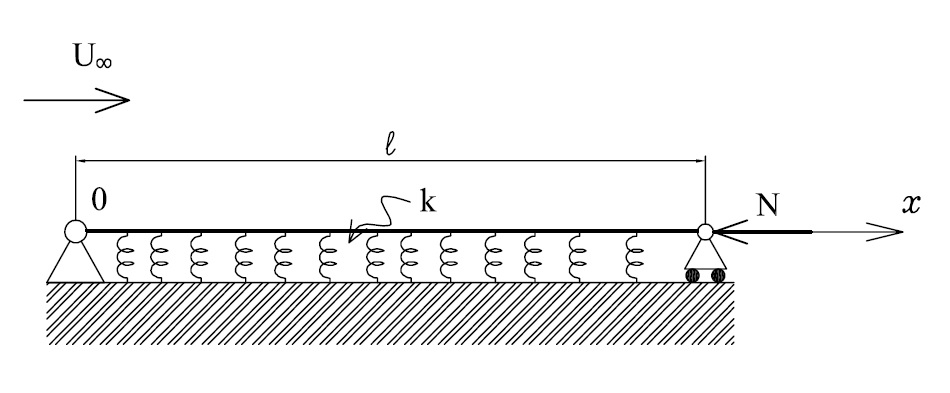
\includegraphics[width=100mm]{Immagini/pannello}
\caption{Pannello soggetto a flusso supersonico}
\end{figure}

\section{Formulazione del problema}
L'equazione del pannello infinito in una direzione, semplicemente appoggiato con carico di punta, e investito nella direzione finita da una corrente supersonica �:\\
 $$EI(1+\zeta\dfrac{\partial}{\partial t})w^{''''} +Nw^{''}+\lambda w^{'}+kw=-\bar{\rho}\ddot{w}-\mu\dot{w}+p(x,t)$$\\
dove $EI$ rappresenta la rigidezza flessionale della trave, $\zeta$ lo smorzamento strutturale, $N$ il carico di punta,
$\lambda$ un coefficiente aerodinamico fornito dalla teoria di Ackeret, $\mu$ uno smorzamento aerodinamico, $k$
la costante del suolo elastico, $\bar{\rho}$ la densit� (lineare) della trave e $p(x,t)$ un carico esterno applicato.\\
Il modello viene discretizzato tramite le autofunzioni $\phi_{n}$ ottenute dal problema delle autosoluzioni dell'operatore strutturale $L_{s}$.\\
E' possibile dimostrare, infatti, che tali autofunzioni sono funzioni indipendenti e ortogonali tra loro e quindi costituiscono una base di proiezione per il teorema di Fourier generalizzato.\\
Bisogna sottolineare come il problema delle autofunzioni associato all'operatore strutturale, $L_{s}\phi_{n}=\lambda_{n}\phi_{n}$ con $\lambda_{n}$ autovalore, consta delle condizioni al contorno.\\
In particolare nel nostro caso si dimostra che la generica $\phi_{n}=\sin(\dfrac{n\pi x}{l})$, essendo l la lunghezza finita del pannello in questione.\\
Procedendo in questo modo si ottiene una rappresentazione esatta della nostra incognita w(x,t):\\
$$w(x,t)=\sum\limits_{n=1}^{\infty} w_{n}(t)\phi_{n}(x)$$\\
troncando la sommatoria al secondo termine $N_{max}=2$, e utilizzando il metodo di Galerkin per le soluzioni in forma debole, otteniamo un sistema di 2 equazioni nelle 2 incognite $w_{1}(t)$ $w_{2}(t)$.\\\\

 
 


\section{Stabilit�}
In questa sezione si proceder� con l'analisi di stabilit� del sistema, attraverso l'uso del luogo delle radici al variare di $\Lambda$.\\
Il calcolo del luogo delle radici verr� reiterato, variando lo smorzamento del sistema stesso, passando da una situazione di struttura non smorzata ad una smorzata, mettendo in evidenza, laddove fosse necessario, le principali differenze che i due casi presentano.\\



\subsection{Caso non smorzato}
Il primo caso analizzato, riguarda il sistema privo di smorzamento, $\zeta_{1}=\zeta_{2}=0$, avendo posto $f_{1}=15$ $Hz$, $f_{2}=30$ $Hz$.\\
L'analisi della stabilit� viene condotta attraverso lo studio del luogo delle radici al variare del parametro $\Lambda$; si ricordi che $\Lambda$ � intimamente connesso alla pressione dinamica del fluido e quindi alla velocit� che esso assume.\\
Si cerca quindi di caratterizzare il sistema in termini di stabilit� aeroelastica al fine di individuarne la condizione critica, che ricordiamo essere dovuta ad una coalescenza dei poli e quindi una risposta divergente del sistema di tipo lineare.\\
 Si riportano i risulati ottenuti:\\
\begin{figure}[htbp!]
	\centering	
	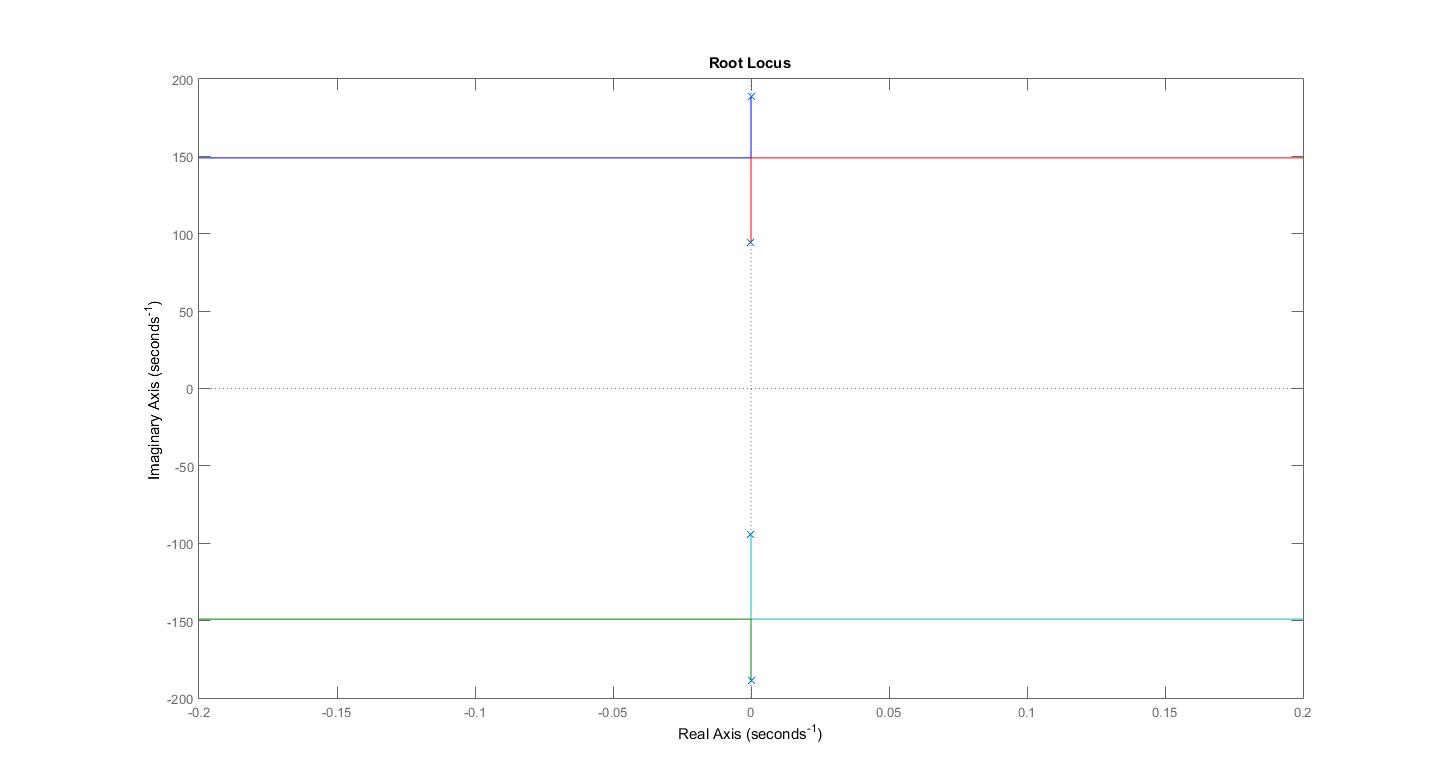
\includegraphics[width=100mm]{Immagini/nosmorz}
	\caption{Luogo delle radici, caso non smorzato}
\end{figure}\\
Si osserva come i poli del sistema associati al primo e secondo modo, in assenza di flusso $\Lambda=0$ (indicati con x in figura), coalescono,per un certo $\Lambda=\Lambda_{cr}$ dando origine all'istabilit� aeroelastica denominata flutter.
Ricordiamo come, in assenza di smorzamento $\Lambda_{cr}$ � direttamente collegato alle frequenze proprie del sistema:\\
$$\Lambda_{cr}=|\dfrac{\omega_{1}^{2}-\omega_{2}^{2}}{2}|$$\\
dove $\omega_{n}=2\pi f_{n}$.\\
Nel nostro caso si ottiene:\\
$$\Lambda_{cr}=13323.96 s^{-2}$$
Si nota come tanto pi� le frequenze proprie sono separate fra loro, tanto pi� l'insorgere del fenomeno del flutter � ritardato.\\
Per completezza si riporta la pulsazione di attraversamento calcolata analiticamente.\\
$$\omega_{cr}^2=\frac{\omega_{1}^2+\omega_{2}^2}{2}$$
ovvero:\\
$$\omega_{cr}=149.02 rad/s$$
Per quanto riguarda quella ottenuta numericamente si ha:
$$\omega_{cr}=149.1 rad/s$$

\subsection{Caso smorzato}
Un altro caso analizzato, � lo studio della stabilit� del sistema in presenza di smorzameto. In particolare verranno analizzate tre configurazioni:\\\\
$\bullet$\quad $\zeta_{1}>\zeta_{2}$\quad\quad\quad\quad $\zeta_{1}=0.03$ e $\zeta_{2}=0.01$ ($s^{-1}$)\\
$\bullet$\quad $\zeta_{1}<\zeta_{2}$\quad\quad\quad\quad $\zeta_{1}=0.03$ e $\zeta_{2}=0.05$ ($s^{-}$)\\
$\bullet$\quad $\zeta_{1}=\zeta_{2}=\zeta$\quad\quad $\zeta=0.03$ ($s^{-1}$)\\\\
Viene ora riportato l'andamento del luogo delle radici la variare del parametro $\Lambda$, per ognuno dei tre sottocasi presi in considerazione.\\
$\bullet$\quad {\bf Caso }$\zeta_{1}>\zeta_{2}$\\\\
\begin{figure}[htbp]
	\centering	
	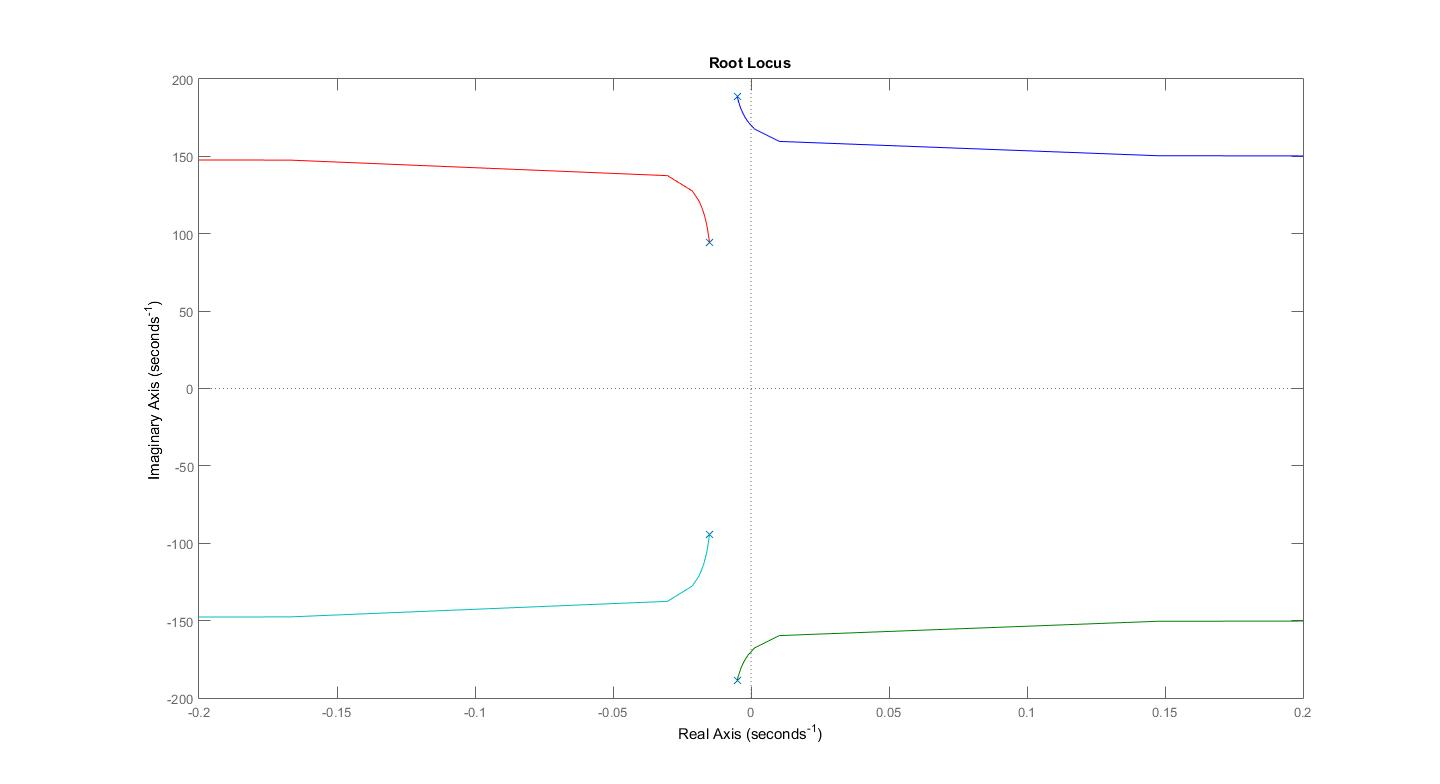
\includegraphics[width=100mm]{Immagini/smorzzita1}
	\caption{Luogo delle radici, caso smorzato $\zeta_{1}>\zeta_{2}$ }
\end{figure}\\
Si nota come i poli in presenza di smorzamento, presentano una parte reale non nulla in assenza di flusso $\Lambda=0$, indicati con x in figura.\\
All'aumentare di $\Lambda$, si vede come i poli tendono inizialmente a coalescere, muovendosi parallalelamente all'asse immaginario, per poi allontanarsi in direzione parallela all'asse reale e in verso opposto.\\ Si nota come il polo associato al minor smorzamento tenda, per un certo valore di $\Lambda$ , ad attraversare l'asse immaginario.\\
 Nel momento in cui l'asse immaginario viene attraversato si ha l'insorgenza di una radice a parte reale positiva, e quindi di un moto di natura divergente (flutter).
 \newpage
$\bullet$\quad {\bf Caso }$\zeta_{1}<\zeta_{2}$ \\\\
\begin{figure}[htbp]
	\centering	
	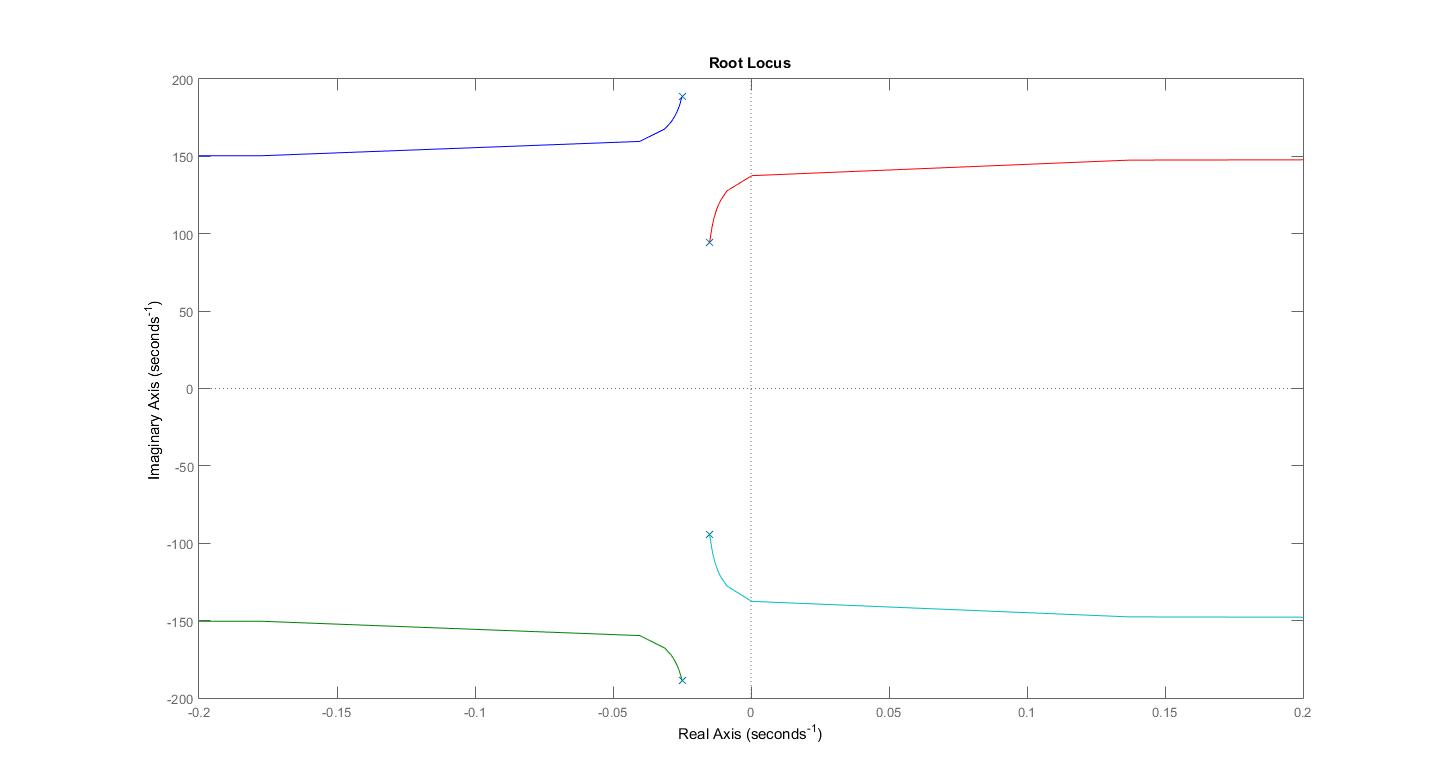
\includegraphics[width=100mm]{Immagini/smorzzita2}
	\caption{Luogo delle radici, caso smorzato $\zeta_{1}<\zeta_{2}$ }
\end{figure}\\
Per quanto riguarda la configurazione con  $\zeta_{1}<\zeta_{2}$, l'andamento � analogo al caso precedente; anche in questo caso la radice a minor smorzamento tende ad attraversare l'asse immaginario con conseguente cambio di segno della parte reale e quindi l'insorgenza di un moto dinamicamente instabile, si veda figura.\\
$\bullet$\quad {\bf Caso }$\zeta_{1}=\zeta_{2}=\zeta$ \\\\
\begin{figure}[htbp]
	\centering	
	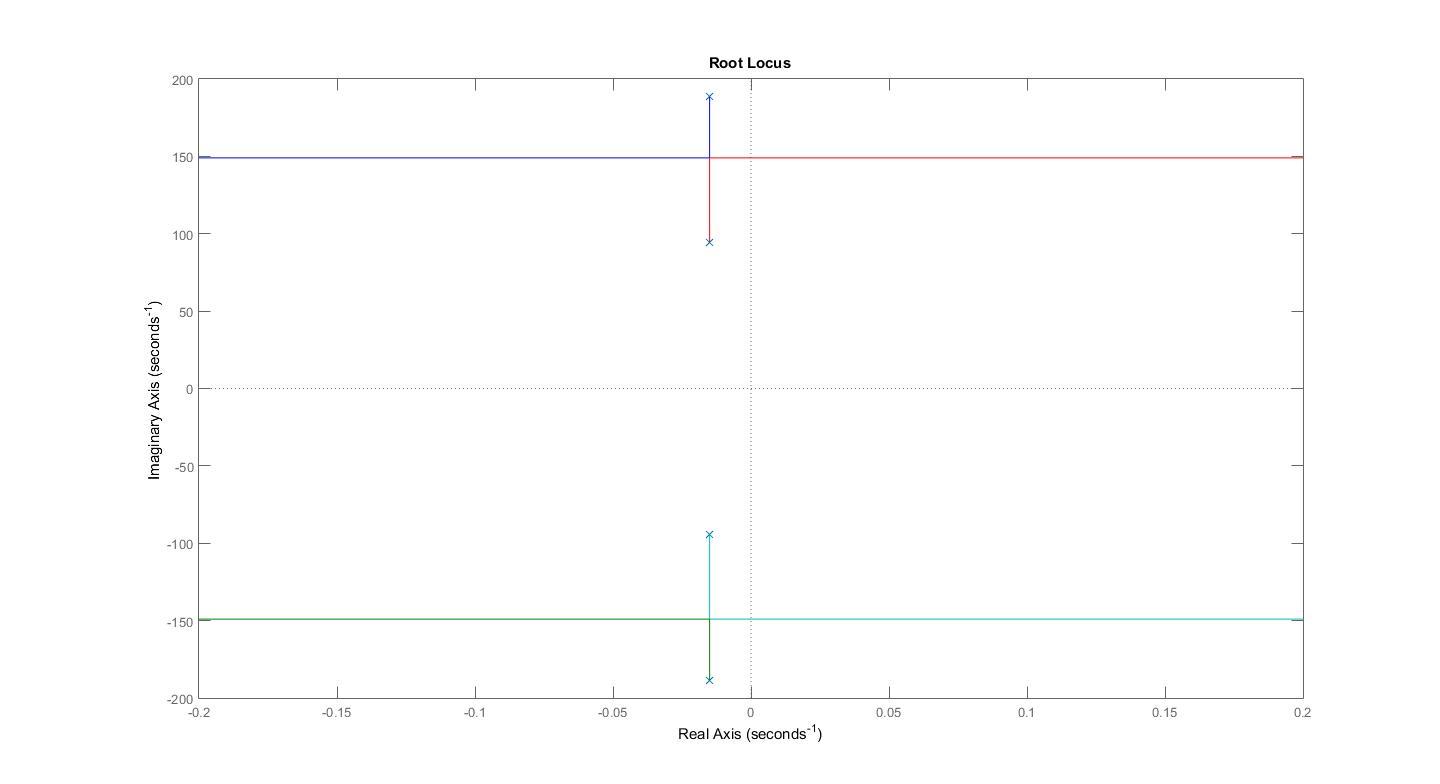
\includegraphics[width=100mm]{Immagini/smorzequal}
	\caption{Luogo delle radici, caso smorzato $\zeta_{1}=\zeta_{2}=\zeta$ }
\end{figure}\\
Si nota un'andamento molto differente ai casi smorzanti precedentemente trattati; infatti l'andamento mostra una somiglianza col caso di sistema non smorzato, ad eccezione che la coalescenza non avviene sull'asse reale ma su un asse parallelo a questo e distante di una quantit� pari a $\dfrac{\zeta}{2}$, questo implica un ritardo nell'insorgere della condizione critica poich� in questo caso la presenza dello smorzamento garantisce una risposta stabile nel punto di coalescenza delle radici. \\
Si nota inoltre come la pulsazione per la quale avviene l'attraversamento dell'asse immaginario sia la stessa del caso di sistema non smorzato.\\
Si riportano in tabella, per i diversi casi, il valore ottenuto dei diversi $\Lambda_{cr}$.\\
\begin{center}
	\begin{tabular}{c c c c}
		\hline
		$\zeta_{1}$ ($s^{-1}$) &$\zeta_{2}$ ($s^{-1}$)&$\Lambda_{cr}$ ($s^{-2}$) &$\omega_{cr}$ (rad/s)\\
		\hline
		0&       0&       1.33239669$\cdot$$10^{4}$ & 149.10\\
		
		0.03&    0.01&    1.15388933 $\cdot$$10^{4}$ & 172.01\\
		
		0.03&    0.05&    1.29008756 $\cdot$$10^{4}$ & 138.23\\
		
		0.03&    0.03&    1.33239658 $\cdot$$10^{4}$ & 149.10\\
		
		\hline
   \end{tabular}
\end{center}
Si nota come il valore del $\Lambda_{cr}$ per il caso $\zeta_{1}=\zeta_{2}=0.03$ sia molto simile a quello ottenuno in assenza di smorzamento, differendo da quest'ulimo di un ordine pari a $10^{-2}$, dovuto come detto in precedenza alla piccola traslazione che si ha sull'asse reale.\\
Un'altra osservazione interessante � che il caso non smorzato e il caso con smorzamento $\zeta_{1}=\zeta_{2}=0.03$, presentino dei valori di $\Lambda_{cr}$ maggiori rispetto agli altri due casi trattati. Questo implica che nel caso non smorzato, cosi come in presenza di uno smorzamento modale unico, il fenomeno del flutter risulta essere ritardato, garantendo un range di velocit� in cui il pannello  lavora senza incorrere in fenomeni di instabilit�.\\




\section{Risposta libera}
In questa sezione si valuter� la risposta libera del sistema stabile ($\Lambda<\Lambda_{cr}$), con le seguenti condizioni iniziali:\\\\
$\bullet$\quad $w(x,0)=\sin(\dfrac{\pi x}{l})$\\\\
$\bullet$\quad $\dot{w}(x,0)=0$\\\\
I risultati verranno confrontati con quelli che si sarebbero ottenuti dallo stesso sistema non smorzato, e in assenza di flusso $\Lambda=0$.\\
Infine si proceder� con una discussione della risposta libera del sistema non smorzato, in situazioni prossime a quelle critiche.\\


\subsection{Risposta libera sub-critica}
In questa sezione verr� effettuato il calcolo della risposta libera di un sistema stabile ($\Lambda<\Lambda_{cr}$), in particolare verranno analizzato il caso in cui si ha:\\\\
$\bullet$\quad $\zeta_{1}>\zeta_{2}$\quad\quad\quad\quad $\zeta_{1}=0.03$ e $\zeta_{2}=0.01$ ($s^{-1}$)\\\\
I risultati ottenuti,verranno confrontati con quelli che si avrebbero in assenza di smorzamento e di aerodinamica  $\zeta_{1}=\zeta_{2}=0$ ,$\Lambda=0$.\\
Si � scelto di descritizzare il problema, scegliendo come funzioni di forma su cui proiettare il sistema di equazioni, le prime due forme modali $\psi^n(x)=\sin(\frac{n\pi x}{l})$, n=1,2.\\
La risposta libera nel tempo � data da:\\\\
$${\bf w}(t)=\sum_{1}^{2}c_{n}\tilde{{\bf w}}^{n}e^{s_{n}t}+ C.C.$$
dove $s_{n}$, $\tilde{{\bf w}}^{n}$ il corrispondente autovettore e le $c_{n}$ rappresentano le costanti complesse dipendenti dalle condizioni iniziali assegnate; con C.C. si sono indicati i corrispettivi complessi coniugati.\\
Imponendo come condizione iniziale:\\\\
$$w(x,0)=\sin\frac{\pi x}{l}$$
$$\dot{w}(x,0)=0$$\\\\
Implementando oppurtamente su codice MatLab si ricavano i seguenti risultati:\\\\
\begin{center}
	\begin{tabular}{c c}
		\hline
		$\Lambda_{cr}$ & $\Lambda_{sub cr}$ \\
		\hline
		1.1538$\cdot$$10^{4}$
		& 
		1.03850$\cdot10^{4}$ \\ 
		\hline
	\end{tabular}
\end{center}

\begin{center}
	\begin{tabular}{c}
		\hline
		$s_{n}$ \\
		\hline
		
		-0.00201 + 174.79i\\
		-0.00201 - 174.79i\\
		-0.01798 + 117.72i\\
		-0.01798 - 117.72i\\
		
		\hline
	\end{tabular}
\end{center}
\begin{center}
	\begin{tabular}{c}
		\hline
		$c_{n}$ \\
		\hline
		
  0.19485 + 0.0000353i\\
  0.19485 - 0.0000353i\\
  0.40662 - 0.0001178i\\
  0.40662 + 0.0001178i\\
		
		\hline
	\end{tabular}
\end{center}
Vengono riportati in figura la risposta libera della struttura, in funzione del tempo e della x.\\
\begin{figure}[htbp]
	\centering	
	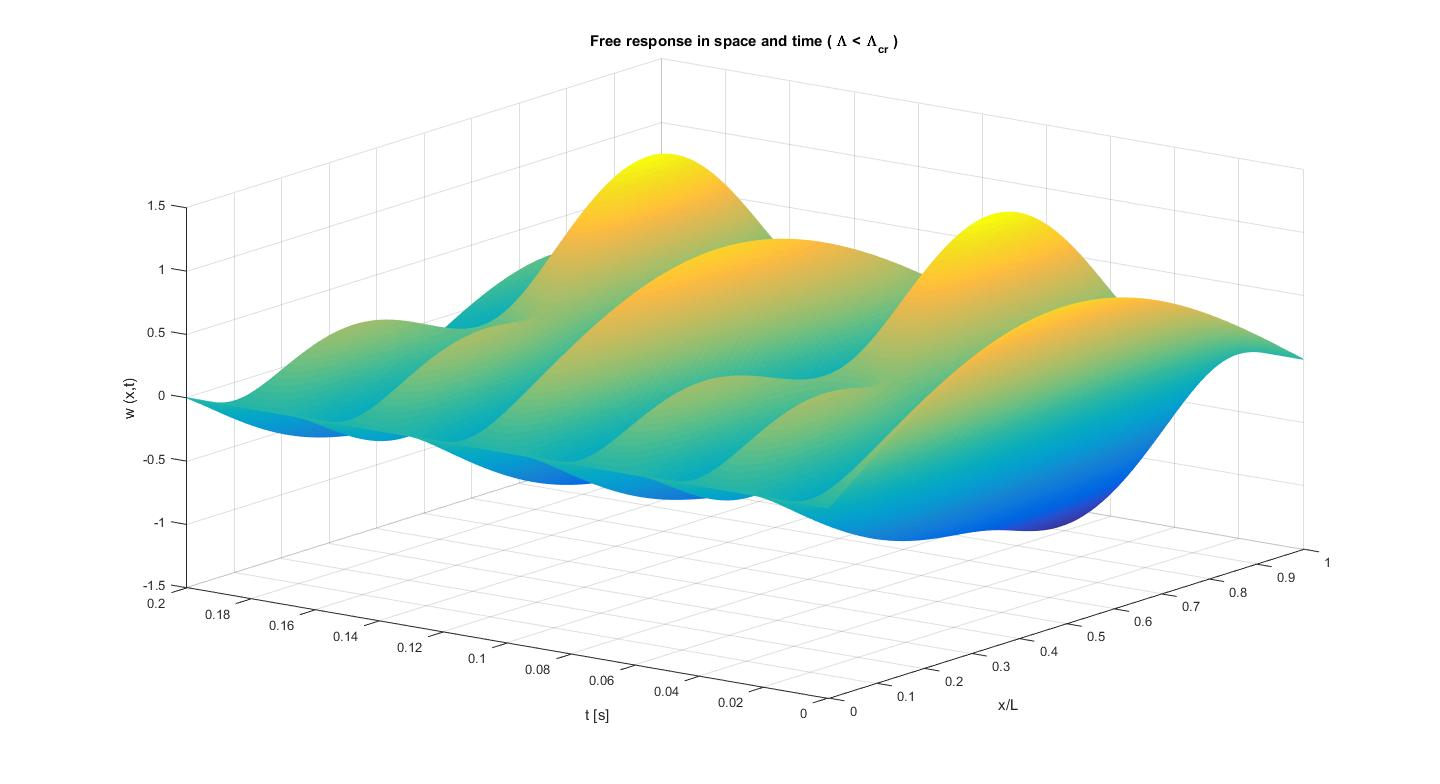
\includegraphics[width=100mm]{Immagini/risposta3daero}
	\caption{Andamento spaziale e temporale 3D del campo di spostamento {\bf w}, caso statible }
\end{figure}\\
Per completezza si riporta la risposta su un piano in funzione di x, per cinque tempi diversi equidistanti tra di loro di $dt=0.02s$, in modo da rendere pi\'u visibile l'evoluzione temporale della risposta\\
\begin{figure}[htbp]
	\centering	
	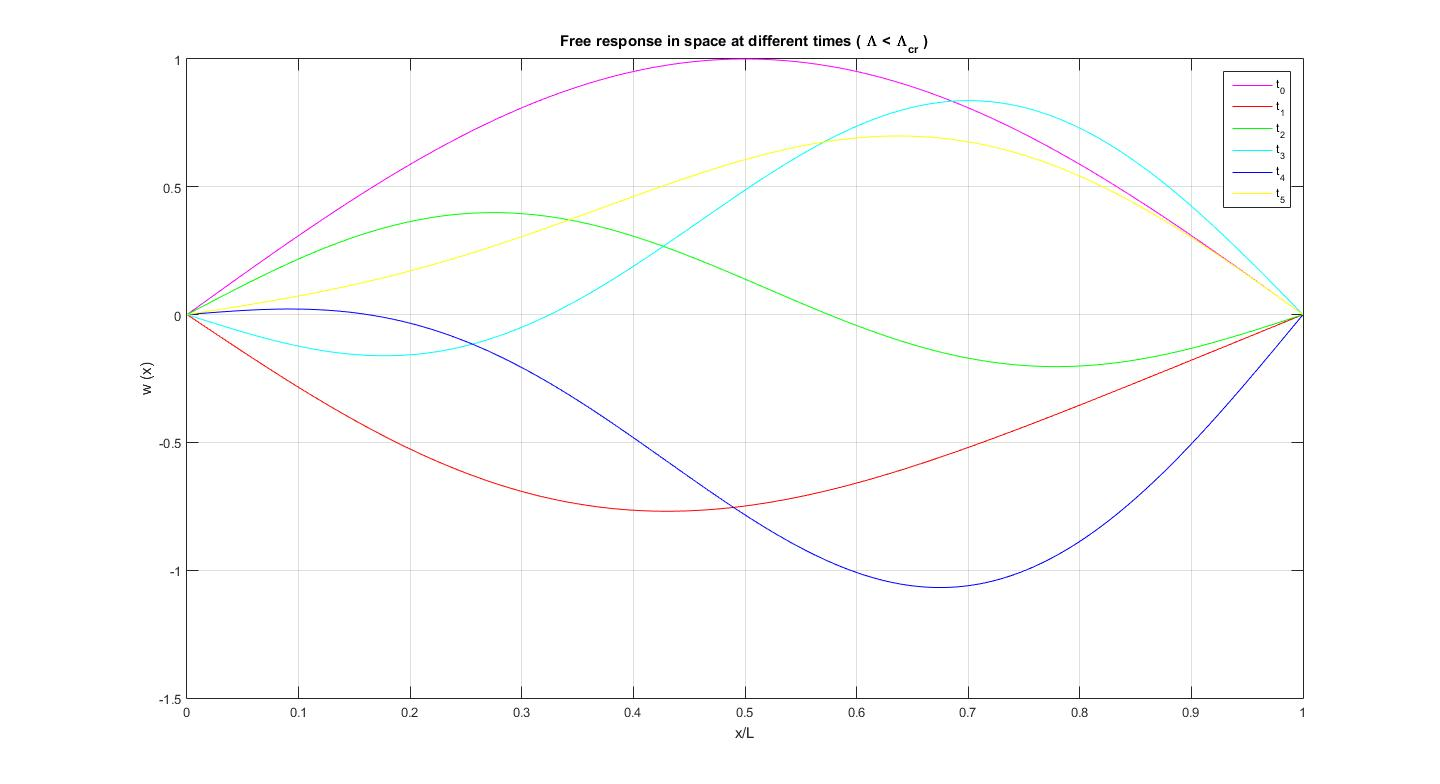
\includegraphics[width=100mm]{Immagini/risposta2daero}
	\caption{Andamento spaziale e temporale 2D del campo di spostamento {\bf w}, caso statible }
\end{figure}\\
Si nota come gli andamenti della risposta libera sia ancora una funzione periodica, che oscilla in tempo ad una determinata frequeza, ma appaia come una combinazione dei modi strutturali sfasati tra loro di una certa quantit�, che si pu� dimostrare essere collegata alle componenti degli autovettori $\tilde{w}$  associati al sistema precedente.\\
Vengono inoltre riportati gli andamenti nel tempo delle $w_{n}(t)\quad n=1,2$,\\\\
\begin{figure}[htbp]
	\subfloat[][\emph{Andamento nel tempo componente $w_{1}(t)$}.]
	{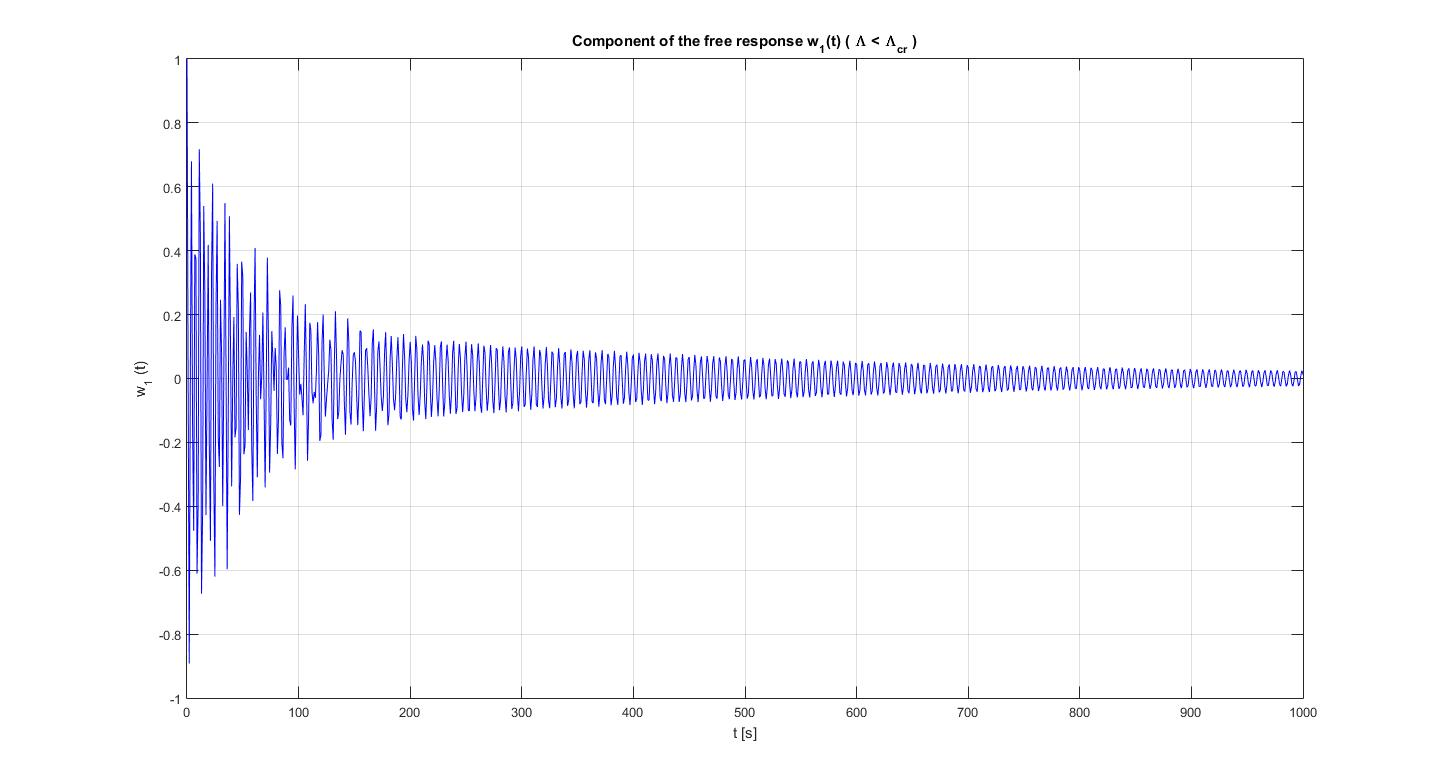
\includegraphics[width=.55\textwidth]{Immagini/w1.jpg}} \quad
	\subfloat[][\emph{Andamento nel tempo componente $w_{2}(t)$}.]
	{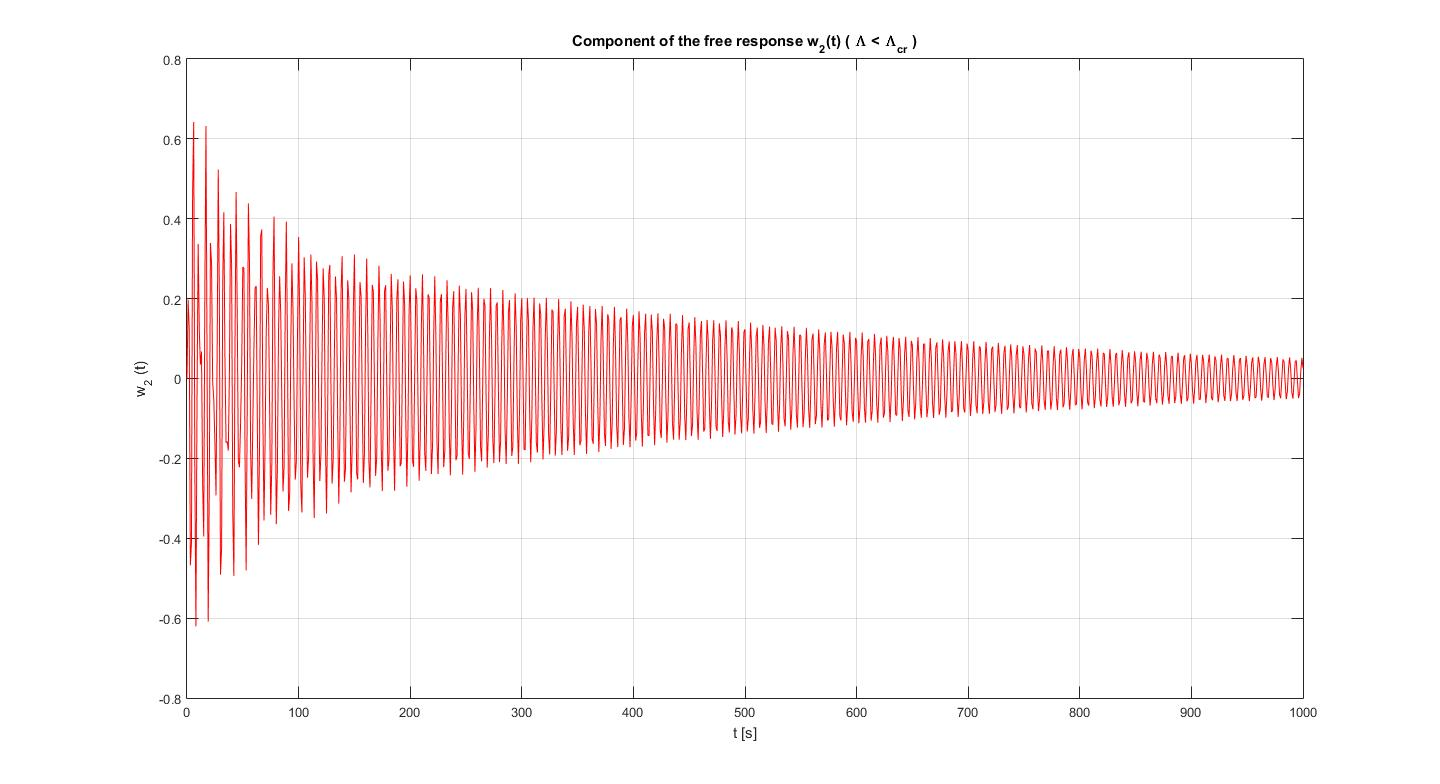
\includegraphics[width=.55\textwidth]{Immagini/w2.jpg}} 
	\label{fig:subfig}
\end{figure}\\
Si nota come le due componenti $w_{n}(t)$ decrescano molto lentamente nel tempo; in particolare la decrescenza della $w_{1}(t)$ risulta maggiore rispetto a quella della componente $w_{2}(t)$.\\
Infine vengono riportati in figura la risposta libera della struttura in assenza di smorzamento e aerodinamica.\\
\begin{figure}[htbp]
	\centering	
	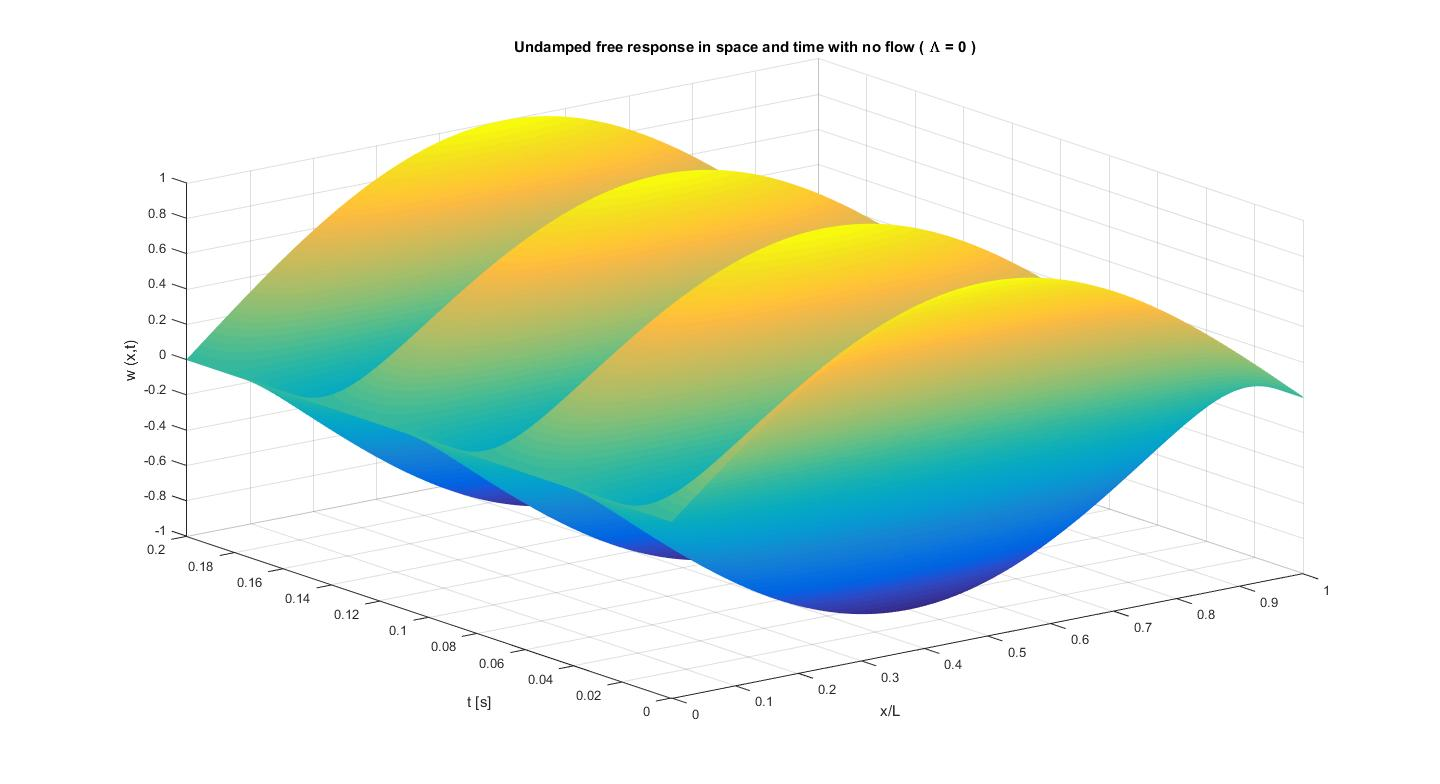
\includegraphics[width=100mm]{Immagini/3dnolambdazita1}
	\caption{Andamento spaziale e temporale 3D del campo di spostamento {\bf w}, no smorzato in assenza di aerodinamica }
\end{figure}\\
Si riporta inoltre la risposta su un piano in funzione di x, avendo messo a parametro il tempo t.\\
\begin{figure}[htbp]
	\centering	
	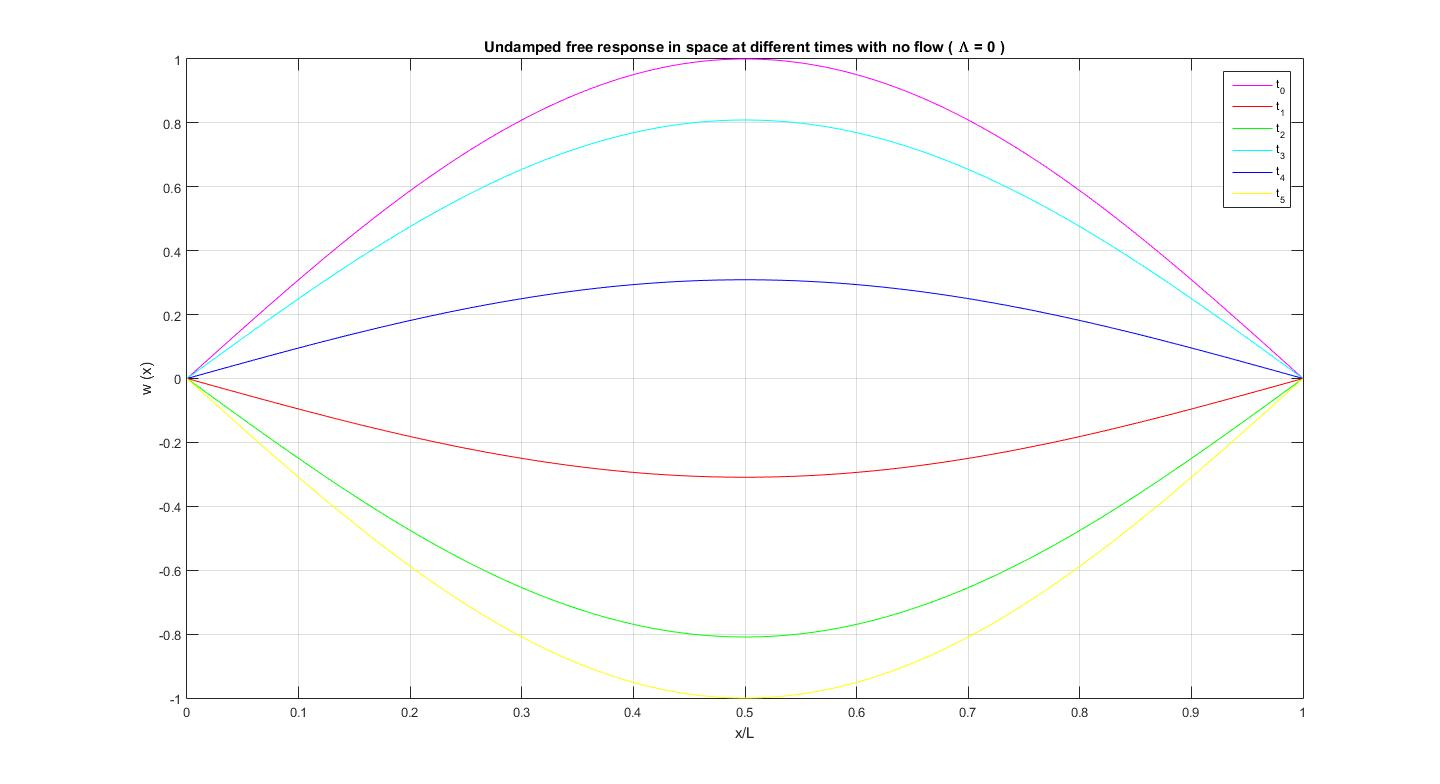
\includegraphics[width=100mm]{Immagini/2dnolambdazita1}
		\caption{Andamento spaziale e temporale 2D del campo di spostamento {\bf w}, no smorzato in assenza di aerodinamica }
\end{figure}
Come ci si aspetta la risposta della stuttura, in ogni punto della stessa, � una risposta di tipo armonico della condizione iniziale $w(x,0)=\sin\frac{\pi x}{l}$, in quanto quest'ultima � uno dei modi propri della struttura stessa per definizione.\\
\newpage 
\subsection{Risposta libera critica}
In questa sezione si cerca di analizzare, almeno in via qualitativa, la risposta libera per il pannello avente $\zeta_{1}=\zeta_{2}=0$ quando $\Lambda\rightarrow\Lambda_{cr}$.\\
Con l'ausilio di uno script in matlab, si � posto $\Lambda=0.999\cdot\Lambda_{cr}$, e si sono calcolate le componenti $w_{n}(t)$, n=1,2.\\
Si riportano i risultati cosi ottenuti:\\
\begin{figure}[htbp]
	\subfloat[][\emph{Andamento nel tempo componente $w_{1}(t)$}.]
	{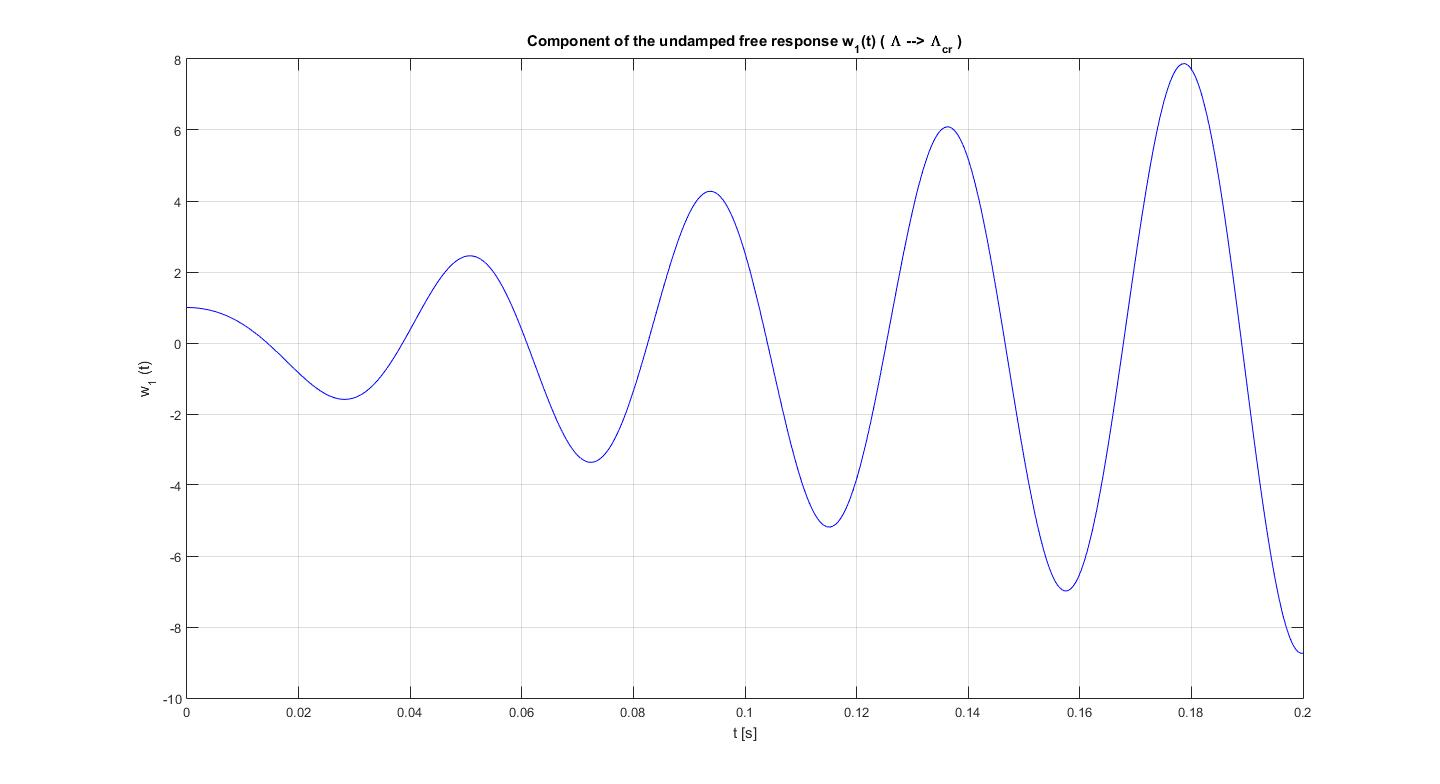
\includegraphics[width=.55\textwidth]{Immagini/w1cr.jpg}} \quad
	\subfloat[][\emph{Andamento nel tempo componente $w_{2}(t)$}.]
	{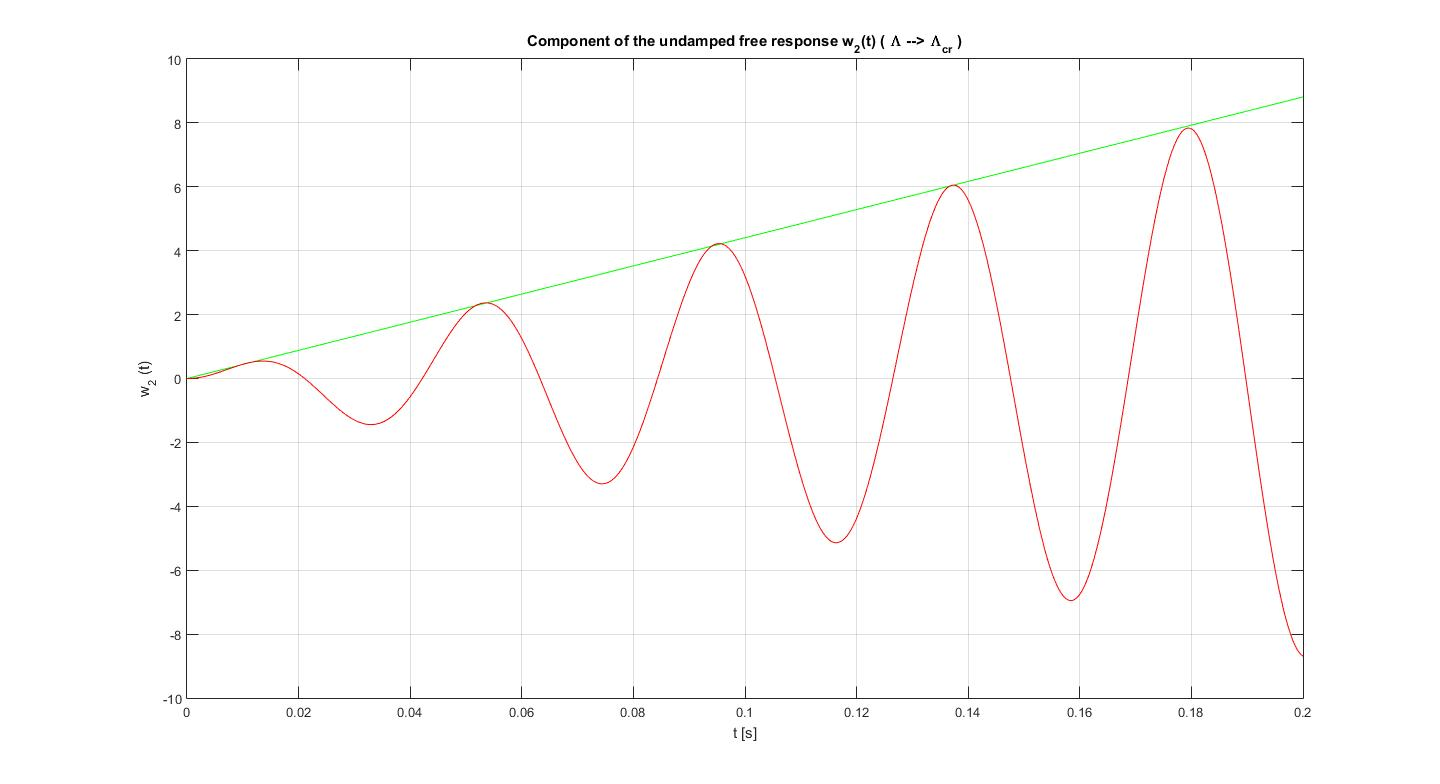
\includegraphics[width=.55\textwidth]{Immagini/w2cr.jpg}} 
	\label{fig:subfig}
\end{figure}\\
Si nota come entrambe le componenti presentano un andamento di tipo oscillatorio, con un inviluppo lineare.\\
Questo fenomeno � tipico della coalescenza dei poli, coalscenza che come ricordiamo avviene sull'asse immaginario.\\
Poich� la molteplicit� geometrica risulta essere uguale a... e in presenza di coalescenza la molteplicit� algebrica risulta uguale a 2, la risposta che si ottiene in questo caso, consta di due termini addizionali, uno armonico semplice e l'altro sempre di natura armonica ma modulato da un inviluppo che � proporzionale a t.\\
Globalmente avremo sempre una risposta armonica data dalla combinazione lineare dei due modi strutturali, che si amplifica al variare del tempo. Il fenomeno � per certi versi simile a quello della risonanza nelle strutture, in cui una forzante esterna forniva energia all'interno della struttura che quest'ultima usava per autoalimentarsi non restituendola. In questo caso, invece, l'energia non � pi� fornita da una forzante esterna bensi dalla corrente di fluido, tuttavia il discorso � analogo a quello della risonanza, in tal senso la struttura si autoeccita fino a divergenza e quindi a collasso.\\ 
 


\end{document}